\documentclass[12pt, block=fill]{beamer}
\usepackage{graphicx}
\usepackage[sfdefault]{FiraSans}
\usepackage{FiraMono}
\usepackage[T1]{fontenc}
\usepackage{xcolor}
\usepackage{mathtools}
\usepackage{txfonts}
\usepackage{ulem}


\usepackage{hyperref}

\definecolor{burntOrange}{rgb}{.8, .5, .1}
\definecolor{textgray}{rgb}{.8,.8,.8}
\definecolor{berkeleyYellow}{HTML}{FDB515}

\usetheme[
titleformat frame = smallcaps,
subsectionpage = progressbar]
{metropolis}

\metroset{
  block=fill
}

\usepackage{pgfpages}
 \setbeameroption{hide notes} % Only slides
% \setbeameroption{show only notes} % Only notes
%  \setbeameroption{show notes on second screen=right} % Both
\setbeamerfont{note page}{size=\footnotesize}

\newcommand{\E}{\text{E}}
\newcommand{\V}{\text{V}}
\newcommand{\cov}{\text{cov}}

\newcommand{\Z}{\mathbb{Z}}
\newcommand{\R}{\mathbb{R}}
\newcommand{\N}{\mathbb{N}}
\newcommand{\paul}[1]{{\color{red}#1}}
\newcommand{\alex}[1]{\textcolor{berkeleyYellow}{#1}}


\title{Week 3}
\subtitle{Summarizing Distributions}

\author{Paul Laskowski and Alex Hughes}
\institute{UC Berkeley, School of Information}

\begin{document}

\begin{frame}
  \maketitle
\end{frame}

\section{The Importance of Summarizing Distributions}

\begin{frame}
  \frametitle{}
    \note[item]{probability distributions are really flexible objects.  that's a great strength because they can represent a lot of different things}
  \note[item]{The number of friends on a social network.}
  
  \center  \hspace{-1cm}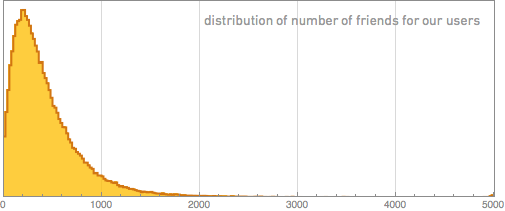
\includegraphics[ width = \textwidth]{images/friends}
  \footnotesize Image: stephenwolfram.com. Data Science of the Facebook World.

\end{frame}

\begin{frame}
  \frametitle{}

  \note[item]{The location of photons in a physics experiment.}
  
  \center  \hspace{-1cm}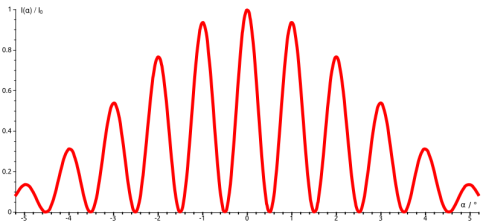
\includegraphics[ width = \textwidth]{images/slit_experiment}

\end{frame}

\begin{frame}
  \frametitle{}
  \note[item]{The liberal or conservative lean of members of congress.}
  
  \center  \hspace{-1cm}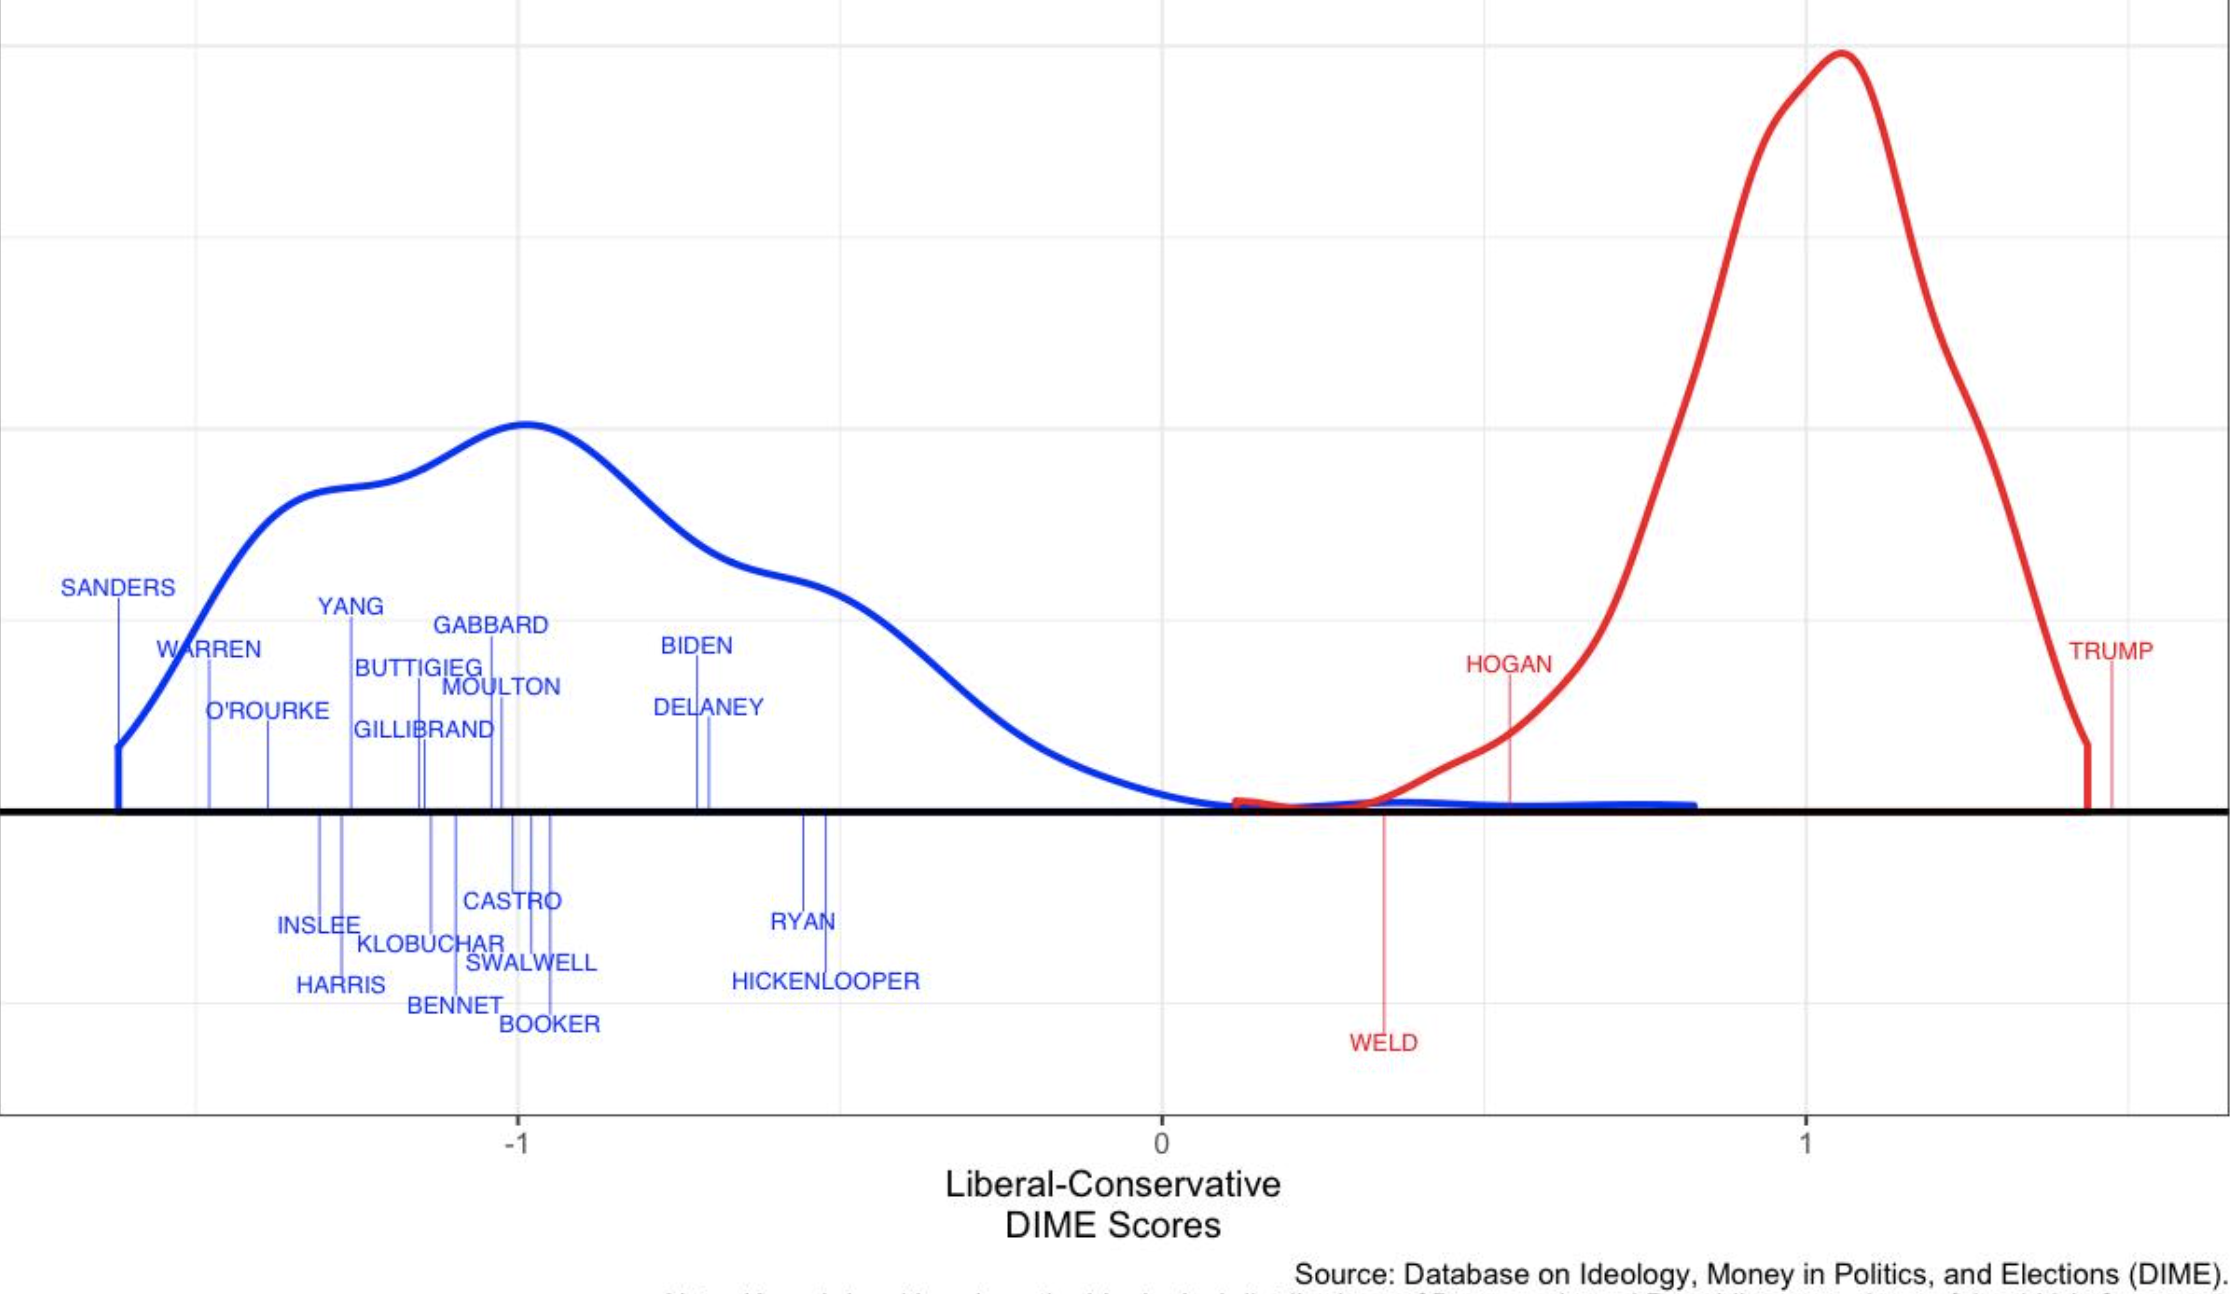
\includegraphics[ width = \textwidth]{images/partisanship}
  
  \note[item]{All of these example only use one random variable, and their distributions have very different shapes.}
  \note[item]{To represent all of these, we need a flexible mathematical object.  We can change a distribution in an infinite number of ways.  move it up a bit in one place, move it down in another.  That's what we need to represent the rich variety of phenomena that we want to model.}
  \note[item]{But there's a down side to all this flexibility...}

\end{frame}






\begin{frame}
  \frametitle{The Downside of Flexibility}

Highly flexible objects present obstacles.
  \begin{itemize}
  \note[item]{Flexibility is great in theory, but how do we actually choose a probability density?}
  \item Cannot specify density for every value \note[item]{we can't select a density for every possible point - that's an infinite number of choices.  and how could I ever communicate those choices to you?}
  \item Cannot communicate or reason about every value
    \note[item]{Even if I could somehow transmit that information to
      you, what could you do with it?}  \note[item]{You can't really
      compare each point of one density against another.}
  \item Cannot estimate density at every value given data
    \note[item]{Finally, you'll want to use data to learn about your
      distribution, but with finite data, you can't estimate density
      at every point.}
  \end{itemize}

  Why not restrict to distributions in a parametric family?
  \begin{itemize}
  \item The real world isn't that neat!
  \item "Agnostic" approach: minimal assumptions on the model
  \end{itemize}
\end{frame}

\begin{frame}
  \frametitle{Why Summarize?}

  \textit{ Summary tools are the hooks we use to estimate, reason
    about, and communicate about random variables.}
\end{frame}

\begin{frame}
  \frametitle{Foundational Summary Tools}
  
  One Random Variable:
\begin{itemize}
\item   Expectation: represents the center of a distribution
\item   Variance: represents the dispersion of a distribution
\end{itemize}

Two Random Variables
\begin{itemize}
\item Covariance: a generalization of variance
\item Correlation: an intuitive measure of linear association
\end{itemize}

  \note[item]{In this unit, we're going to cover a few of the most foundational summary tools out there.}
  \note[item]{We'll start with a single random variable.}
    \note[item]{Expectation, as we'll see, is like a mean, but a version
    of the mean for random variables. Variance is about how spread out a distribution is.}
  \note[item]{Then we'll move on to pairs of random variables - how do we summarize relationships?}
  \note[item]{covariance and correlation are tools that capture the strength of a linear relationship in a single number}
  \note[item]{At the end of this unit, you'll be much better placed to study, and communicate about random varibles.}
\end{frame}



\section{Review of Operators and Functions} 

\begin{frame}
  \frametitle{Review of Operators and Functions}

  \centering
  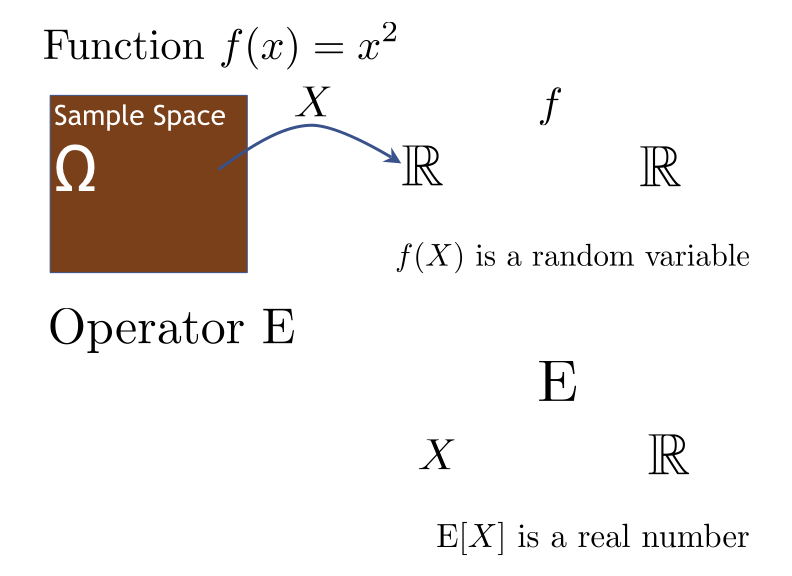
\includegraphics[width=\linewidth]{images/functions_operators}

  
  \note[item]{As you start reading about expectation, it's good to be reminded that expectation is an example of an operator.  Actually, all the summary tools we're going to cover are operators, so let's quick review what that word means.  What's the difference between a function and an operator.}
  \note[item]{When we say a function of a random variable, we mean a
    function from R to R} \note[item]{A function takes the output of a
    random variable as input and maps it to a new real number}
  \note[item]{putting a random variable into a function gives you
    another random variable} \note[item]{Expectation is an
     operator, which means it takes an entire random variable as
    input} \note[item]{So, for example, E[X] is a real number}

\end{frame}


\section{Reading: Summarizing Distributions} 

\begin{frame}
  \frametitle{Reading Assignment}
  Read \textit{Foundations of Agnostic Statistics}, page 44 to the top
  of page 47, stopping after you read theorem 2.1.5.
\end{frame}


\section{Lightboard: Expectation of a Discrete Random Variable}

\begin{frame}
  \frametitle{Expectation of a Discrete Random Variable}
\end{frame}


\begin{frame}
 % \textbf{Note: This is a lightboard. We're just placing it here for
 %   organization.} 
  \frametitle{Expectation for Discrete Random Variables}
  \begin{columns}
    \begin{column}{0.5\textwidth}
      $\E[X] = \sum_{x \in supp[X]} xf(x)$ \note[item]{this is the
        equation for an average, but it's a weighted average.  The
        weight comes from the probability.}
  
      Ex 1 : $X \sim \text{Bernoulli}(\alpha)$
  
      $f(x) = \begin{cases}
        \alpha, & x=1\\
        1-\alpha, & x=0\\
        0, &otherwise
      \end{cases}
      $
  
      $\E[X] = 0 \cdot (1-\alpha) + 1 \cdot \alpha = \alpha$
 
      \note[item]{statisticians like to do this - define things so the
        expectation is the parameter} \note[item]{And the
        interpretation is really useful - the expectation is the
        probability of success}
    \end{column}
    \begin{column}{0.55\textwidth}

      Ex 2: $Y \sim \text{Geometric}(\beta)$

      Let $J_i$ be the event printer jams day $i$.

      $P(J_i) = \beta$, all ind.

      Let $Y$ be days until first jam $P(Y=1) = P(J_1) = \beta$
      $P(Y=2) = P( J_1^C, J_2 ) = (1-\beta) \beta $
      $P(Y=3) = (1-\beta)^2 \beta$

      $f(x) = \begin{cases}
        (1-\beta)^{x-1}\beta , & x \in \{1,2...\} \\
        0, &otherwise
      \end{cases}
      $


      $\E[Y] = \sum_{x = 1}^\infty x (1-\beta)^{x-1} \beta $
      $ = 1/\beta $
    \end{column}
  \end{columns}
\end{frame}

\section{Lightboard: Expectation of a Continuous Random Variable} 
\begin{frame}[t]
  \frametitle{Expectation of a Continuous Random Variable}
    \hspace{4cm} 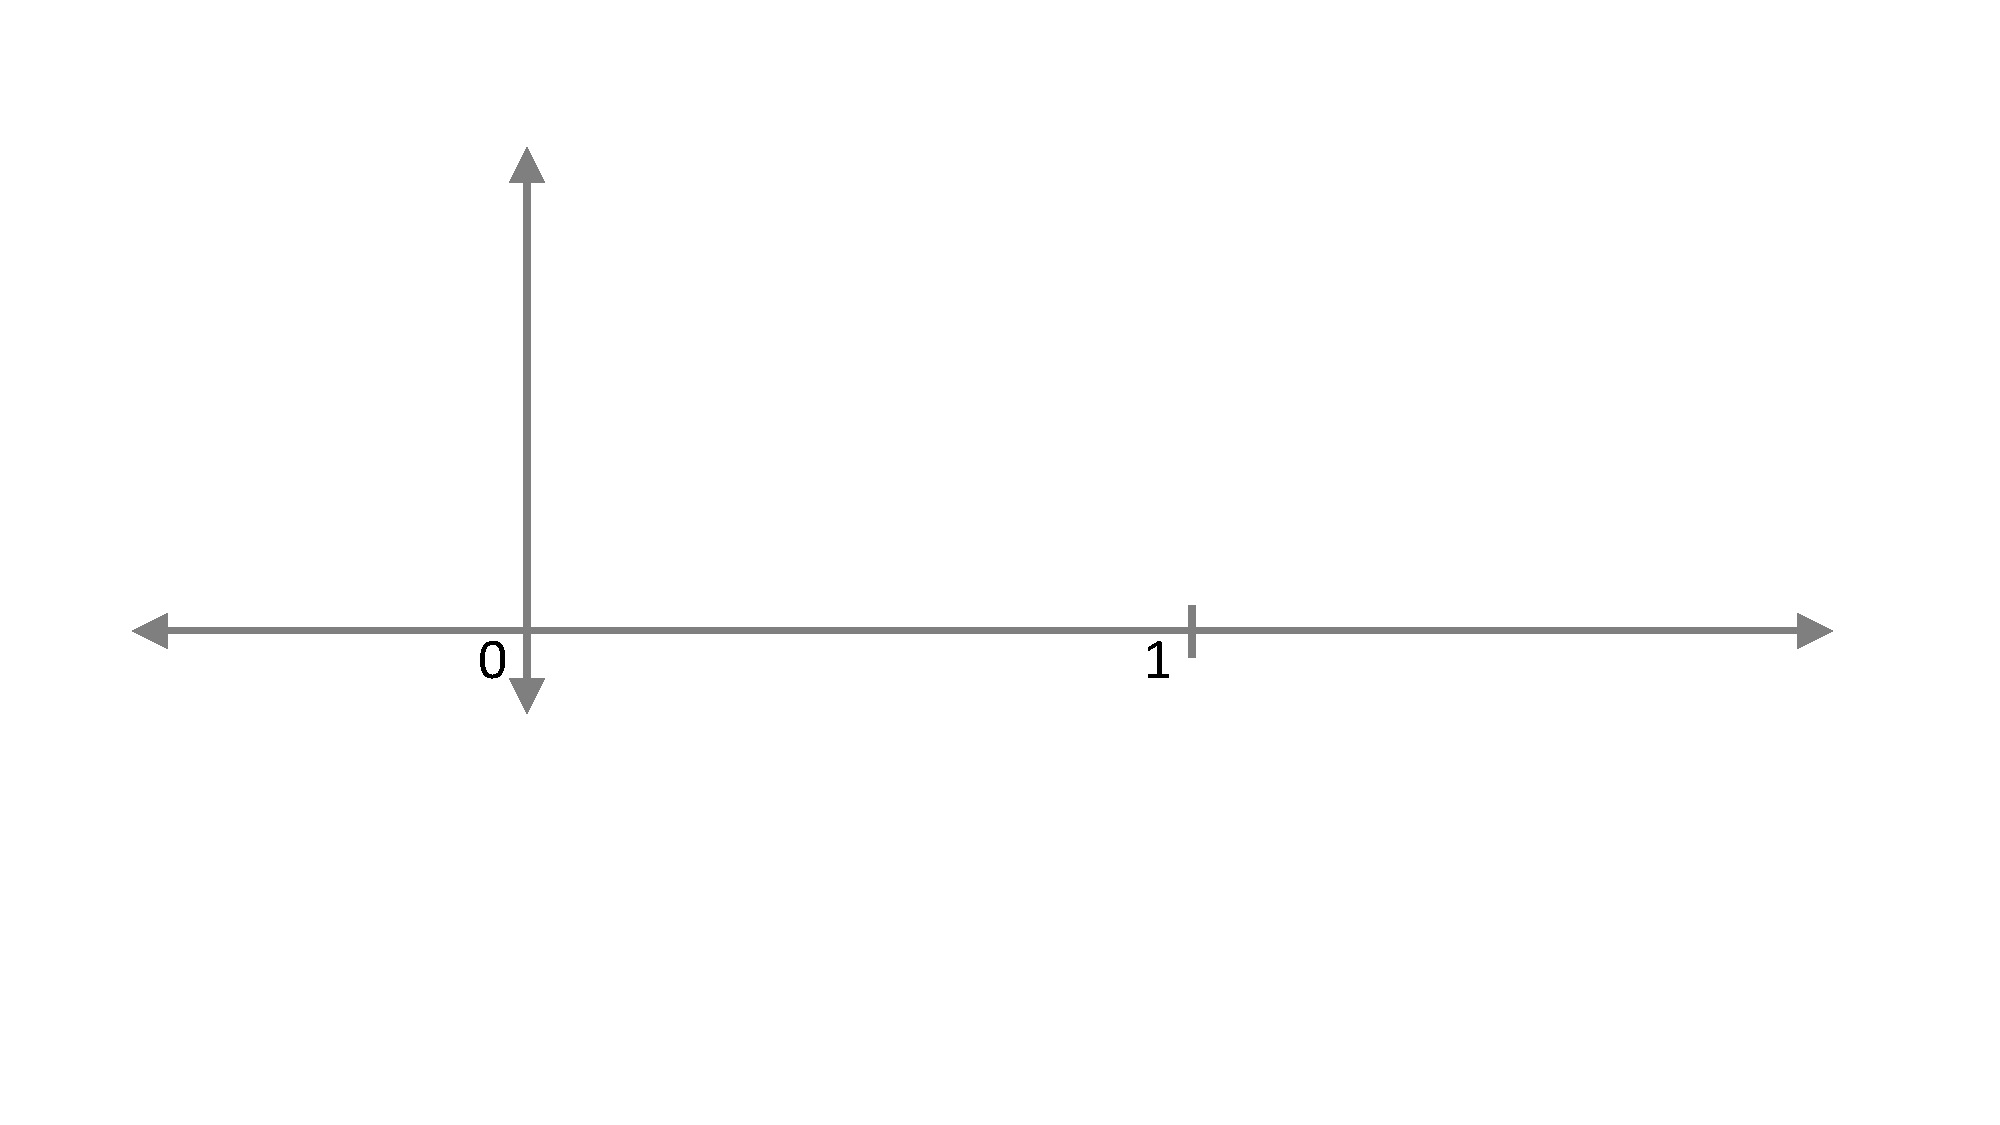
\includegraphics[ width = .6\textwidth]{images/axes}

\end{frame}


\begin{frame}
  \frametitle{Expectation for Continuous Random Variables}
  
  \begin{columns}
    \begin{column}{0.5\textwidth}
      $\E[X] = \int_{-\infty}^\infty xf(x)dx$
 
      Ex 1: $X \sim \text{Uniform}(a,b)$ \note[item]{\paul{did we
          definitely introduce uniform random vars earlier?}}
      \note[item]{pre draw uniform dist.}
  
      $f_X(x) = \begin{cases}
        \frac{1}{b-a}, &a<x<b\\
        0, &otherwise
      \end{cases}$

      $\E[X] = \int_{-\infty}^\infty xf(x)dx$
  
      $ = \int_{-\infty}^a x\cdot 0 dx + \int_a^b x \frac{1}{b-a}dx +
      \int_b^\infty x \cdot 0dx$
  
      $ = 0 + \frac{x^2}{2} \frac{1}{b-a} |_a^b + 0 $
 
      $ = \frac{b^2- a^2}{2} \frac{1}{b-a} = \frac{(b-a) (b+a)}{2}
      \frac{1}{b-a} $
 
      $=\frac{a+b}{2}$

    \end{column}
    \begin{column}{0.5\textwidth}

    \end{column}
  \end{columns}
\end{frame}

\section{Law of the Unthinking Statistician} 

\begin{frame}[t]
  \frametitle{Law of the Unthinking Statistician (LOTUS)}
    \hspace{-1cm}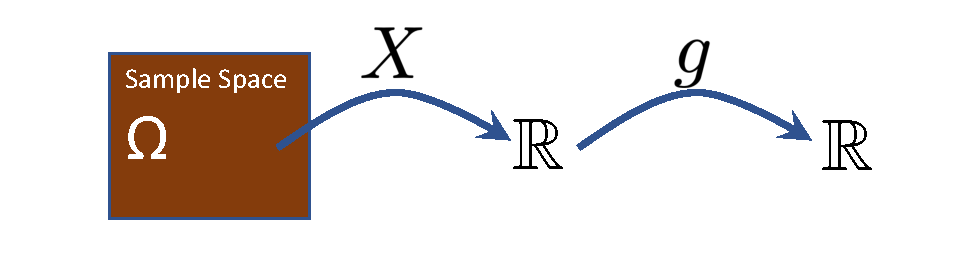
\includegraphics[ width = .7\textwidth]{images/lotus}
  \end{frame}


\begin{frame}[t]
  \frametitle{Law of the Unthinking Statistician (LOTUS)}
  \hspace{-1cm}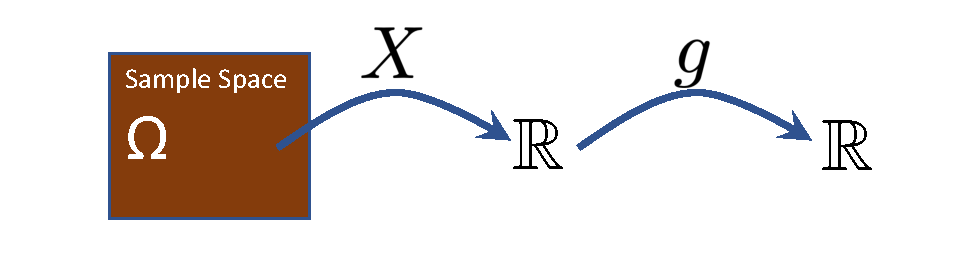
\includegraphics[ width = .7\textwidth]{images/lotus}
  
  \begin{columns}
    \begin{column}{0.5\textwidth}
      X is a DRV with pmf $f$
      
      g(X) is a DRV with pmf,
      
      $f'(y) = P(g(X) = y) = \sum_{x \in \R : g(x) = y} f(x) $
      
      want: $\E[g(X)]$ \note[item]{We want the expectation of g(X).  we
        could first compute the pmf of g(X) then find the expectation.
        That can be hard.}  \note[item]{Instead, we have this really
        useful formula} \note[item]{This is called LOTUS - I think
        because it's so easy, that once you level up enough as a
        statistician, you don't have to be conscious to apply it}
      
      
      $\E[g(X)] = \sum_x g(x)f(x)$
    \end{column}
    \begin{column}{0.5\textwidth}
      Proof sketch:
      \begin{align*}
        \E[g(X)] &= \sum_y y f'(y) \\ 
                &= \sum_y \sum_{x \in \R : g(x) = y} y f(x) \\ 
                &= \sum_y \sum_{x \in \R : g(x) = y} g(x) f(x) \\ 
                &= \sum_{x \in \text{Supp}[X]} g(x) f(x) \\
      \end{align*}
      
      DRV $X$, $Y$, with joint pmf $f$, $h: \R \rightarrow \R$
      
      $\E[h(X,Y)] = \sum_x \sum_y h(x,y) f(x,y)$
      
    \end{column}
  \end{columns}
\end{frame}

\section{Reading: Linearity of Expectation}

\begin{frame}
  \frametitle{Reading Assignment}
  Read \textit{Foundations of Agnostic Statistics}, pages 47–50,
  stopping at 2.1.2.
\end{frame}


\section{Lightboard: Linearity of Expectation}

\begin{frame}
  \frametitle{Linearity of Expectation}


  \note[item]{We introduced expectation by comparing it to the mean,
    and yes, it is a mean, but that makes it sound like just a fixed
    number} \note[item]{It's important to start thinking about
    expectation as an operator.  from the space of random variables to
    R} \note[item]{As an operator, expectation has important
    properties.  Let's quickly see a few of them}



  \begin{columns}
    \begin{column}{0.5\textwidth}

      Assume RV $C$ with pmf

      $f(x) = \begin{cases}
        1, & x=c\\
        0, &otherwise
      \end{cases}
      $
  
      then $C$ is a constant.

      $\E[C] = \sum_x x f(x) = c f(c) = c$

      *usually write $c$ for RV.

      Let $X$, $Y$ be DRVs.  $a \in \R$ \note[item]{All of these are true
        for discrete and continuous RVs, but we'll prove with discrete
        to make things easy.  the continuous proofs are very similar}

      $\E[aX] = \sum_{x \in Supp[X]} ax f_X(x) = a \sum_{x \in Supp[X]}
      x f_X(x) = a \E[X]$

    \end{column}
    \begin{column}{0.5\textwidth}

      $\E[X + Y] = \sum_{x \in X(\Omega), y \in Y(\Omega)} (x+y)
      f(x,y)$
      $ = \sum_{x} \sum_{y} x f(x,y) + \sum_{y} \sum_{x} y f(x,y) $

      $ = \sum_{x} x \sum_{y} f(x,y) + \sum_{y} y \sum_{x} f(x,y) $

      $ = \sum_{x} x f_X(x) + \sum_{y} y f_Y(y) $

      $= \E[X] + \E[Y]$

    \end{column}
  \end{columns}

\end{frame}

\section{Reading: Moments and Variance} 

\begin{frame}
  \frametitle{Reading Assignment}
  Read \textit{Foundations of Agnostic Statistics}, section 2.1.2.
\end{frame}
    
    
\section{Lightboard: Moments and Variance}

\begin{frame}
  \frametitle{Moments and Variance}
  
  \begin{columns}
    \begin{column}{0.5\textwidth}
      (raw) moments:

      1. $\E[X]$ 2. $\E[X^2]$ 3. $\E[X^3]$...  \note[item]{What do the
        moments measure?  Well, one way to think about them is that as
        the power gets higher, the larger values of X dominate the
        smaller ones, so it's like you're checking for how much
        probability is in the tails.}  \note[item]{\paul{Possibly omit
          moments discussion?  we will refer to them in method of
          moments, but can always review}}

      Define variance.

      % $\V[aX] = E\big[ (aX - \E[aX]) ^2 \big] = E\big[ (aX - a\E[X]) ^2
      % \big] = E\big[ a^2 (X - \E[X]) ^2 \big] = a^2 E\big[ (X - \E[X])
      % ^2 \big] = a^2 \V[X] $


    \end{column}
    \begin{column}{0.5\textwidth}

      $\V[aX] = \E[ (aX)^2 ] - \E[aX]^2 = a^2 \E[X^2] - (a\E[X])^2 = a^2
      \E[X^2] - a^2 \E[X]^2 = a^2 \V[X] $


      $\V[X+ c] = E\big[ (X + c - \E[X + c]) ^2 \big] = \E\big[ (X + c -
      \E[X] -\E[c]) ^2 \big] = \E\big[ (X - \E[X]) ^2 \big] = \V[X] $

      \note[item]{\paul {Chebyshev is in here - but maybe postpone
          till needed for LLN?}}
    \end{column}
  \end{columns}
\end{frame}




\section{Reading: Mean Squared Error (MSE)}

\begin{frame}
  \frametitle{Reading Assignment}
  Read \textit{Foundations of Agnostic Statistics}, section 2.1.3.
\end{frame}
    
\section{Lightboard: Mean Squared Error (MSE)  - Lightboard}

\begin{frame}
  \frametitle{The Expected Value and MSE}
  Proof that $\E[X]$ minimizes MSE

  \note[]{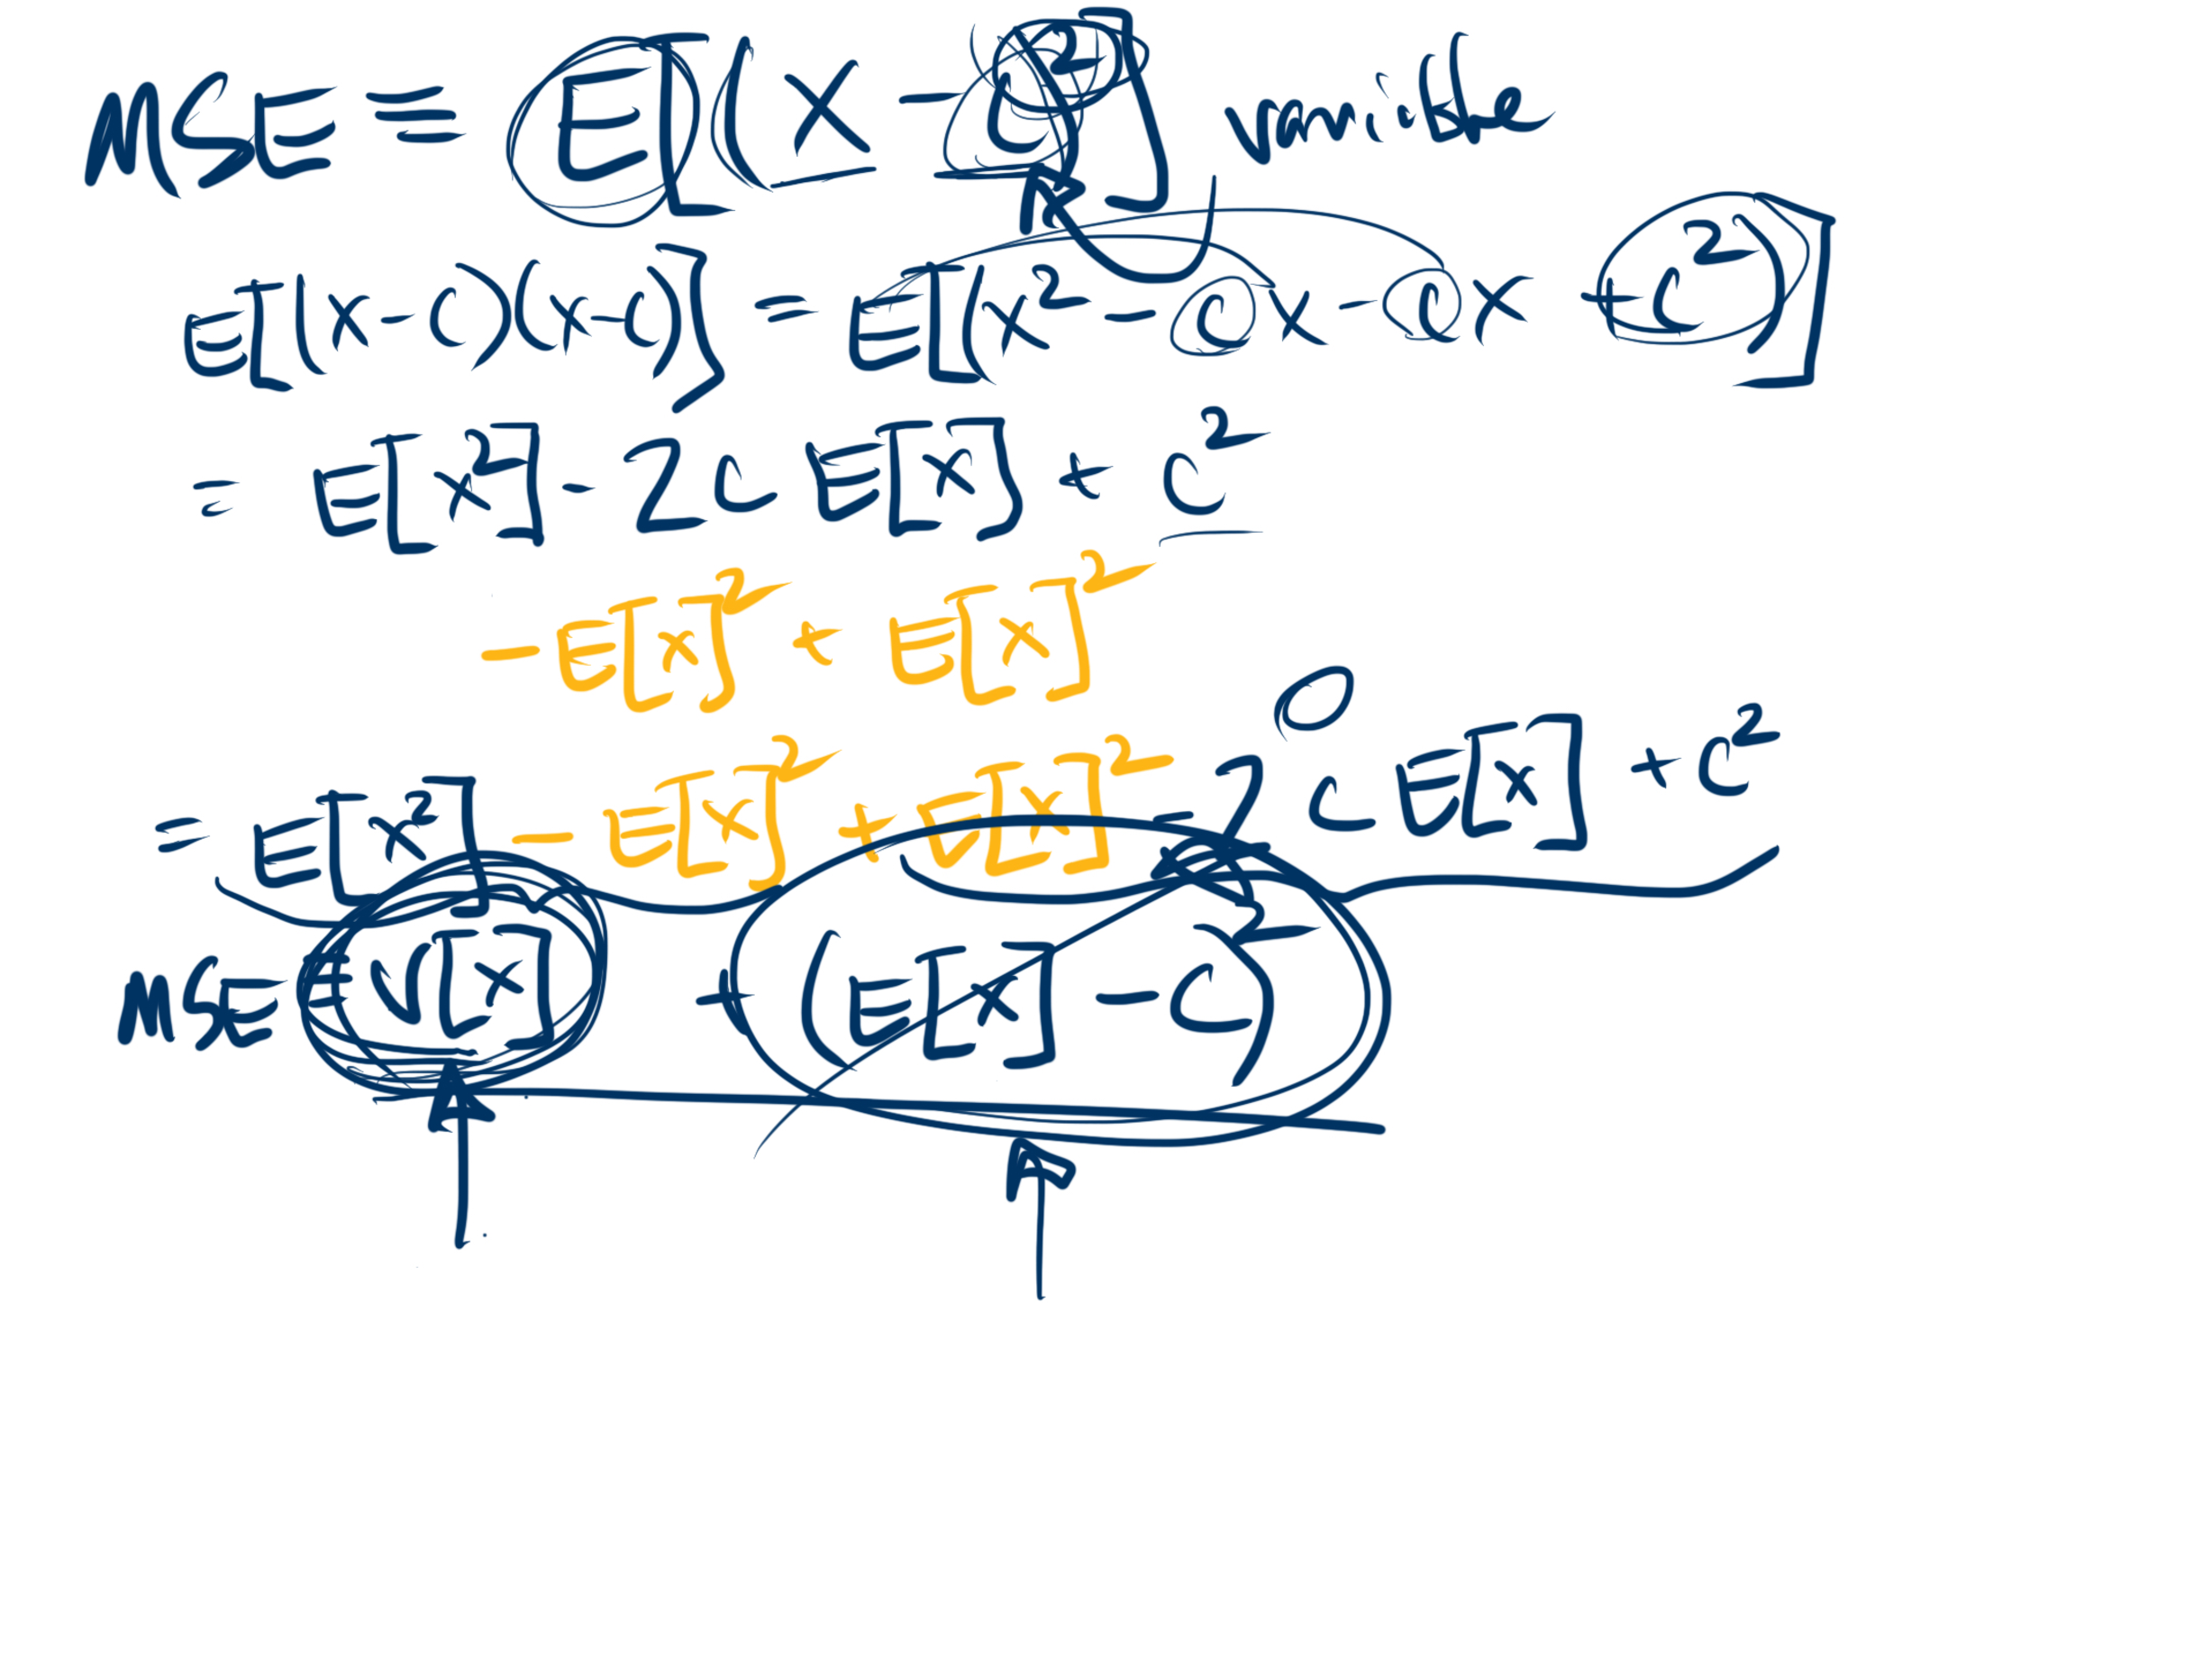
\includegraphics[width=0.3\linewidth]{images/Mean_Squared_Error_1}}
  \note[]{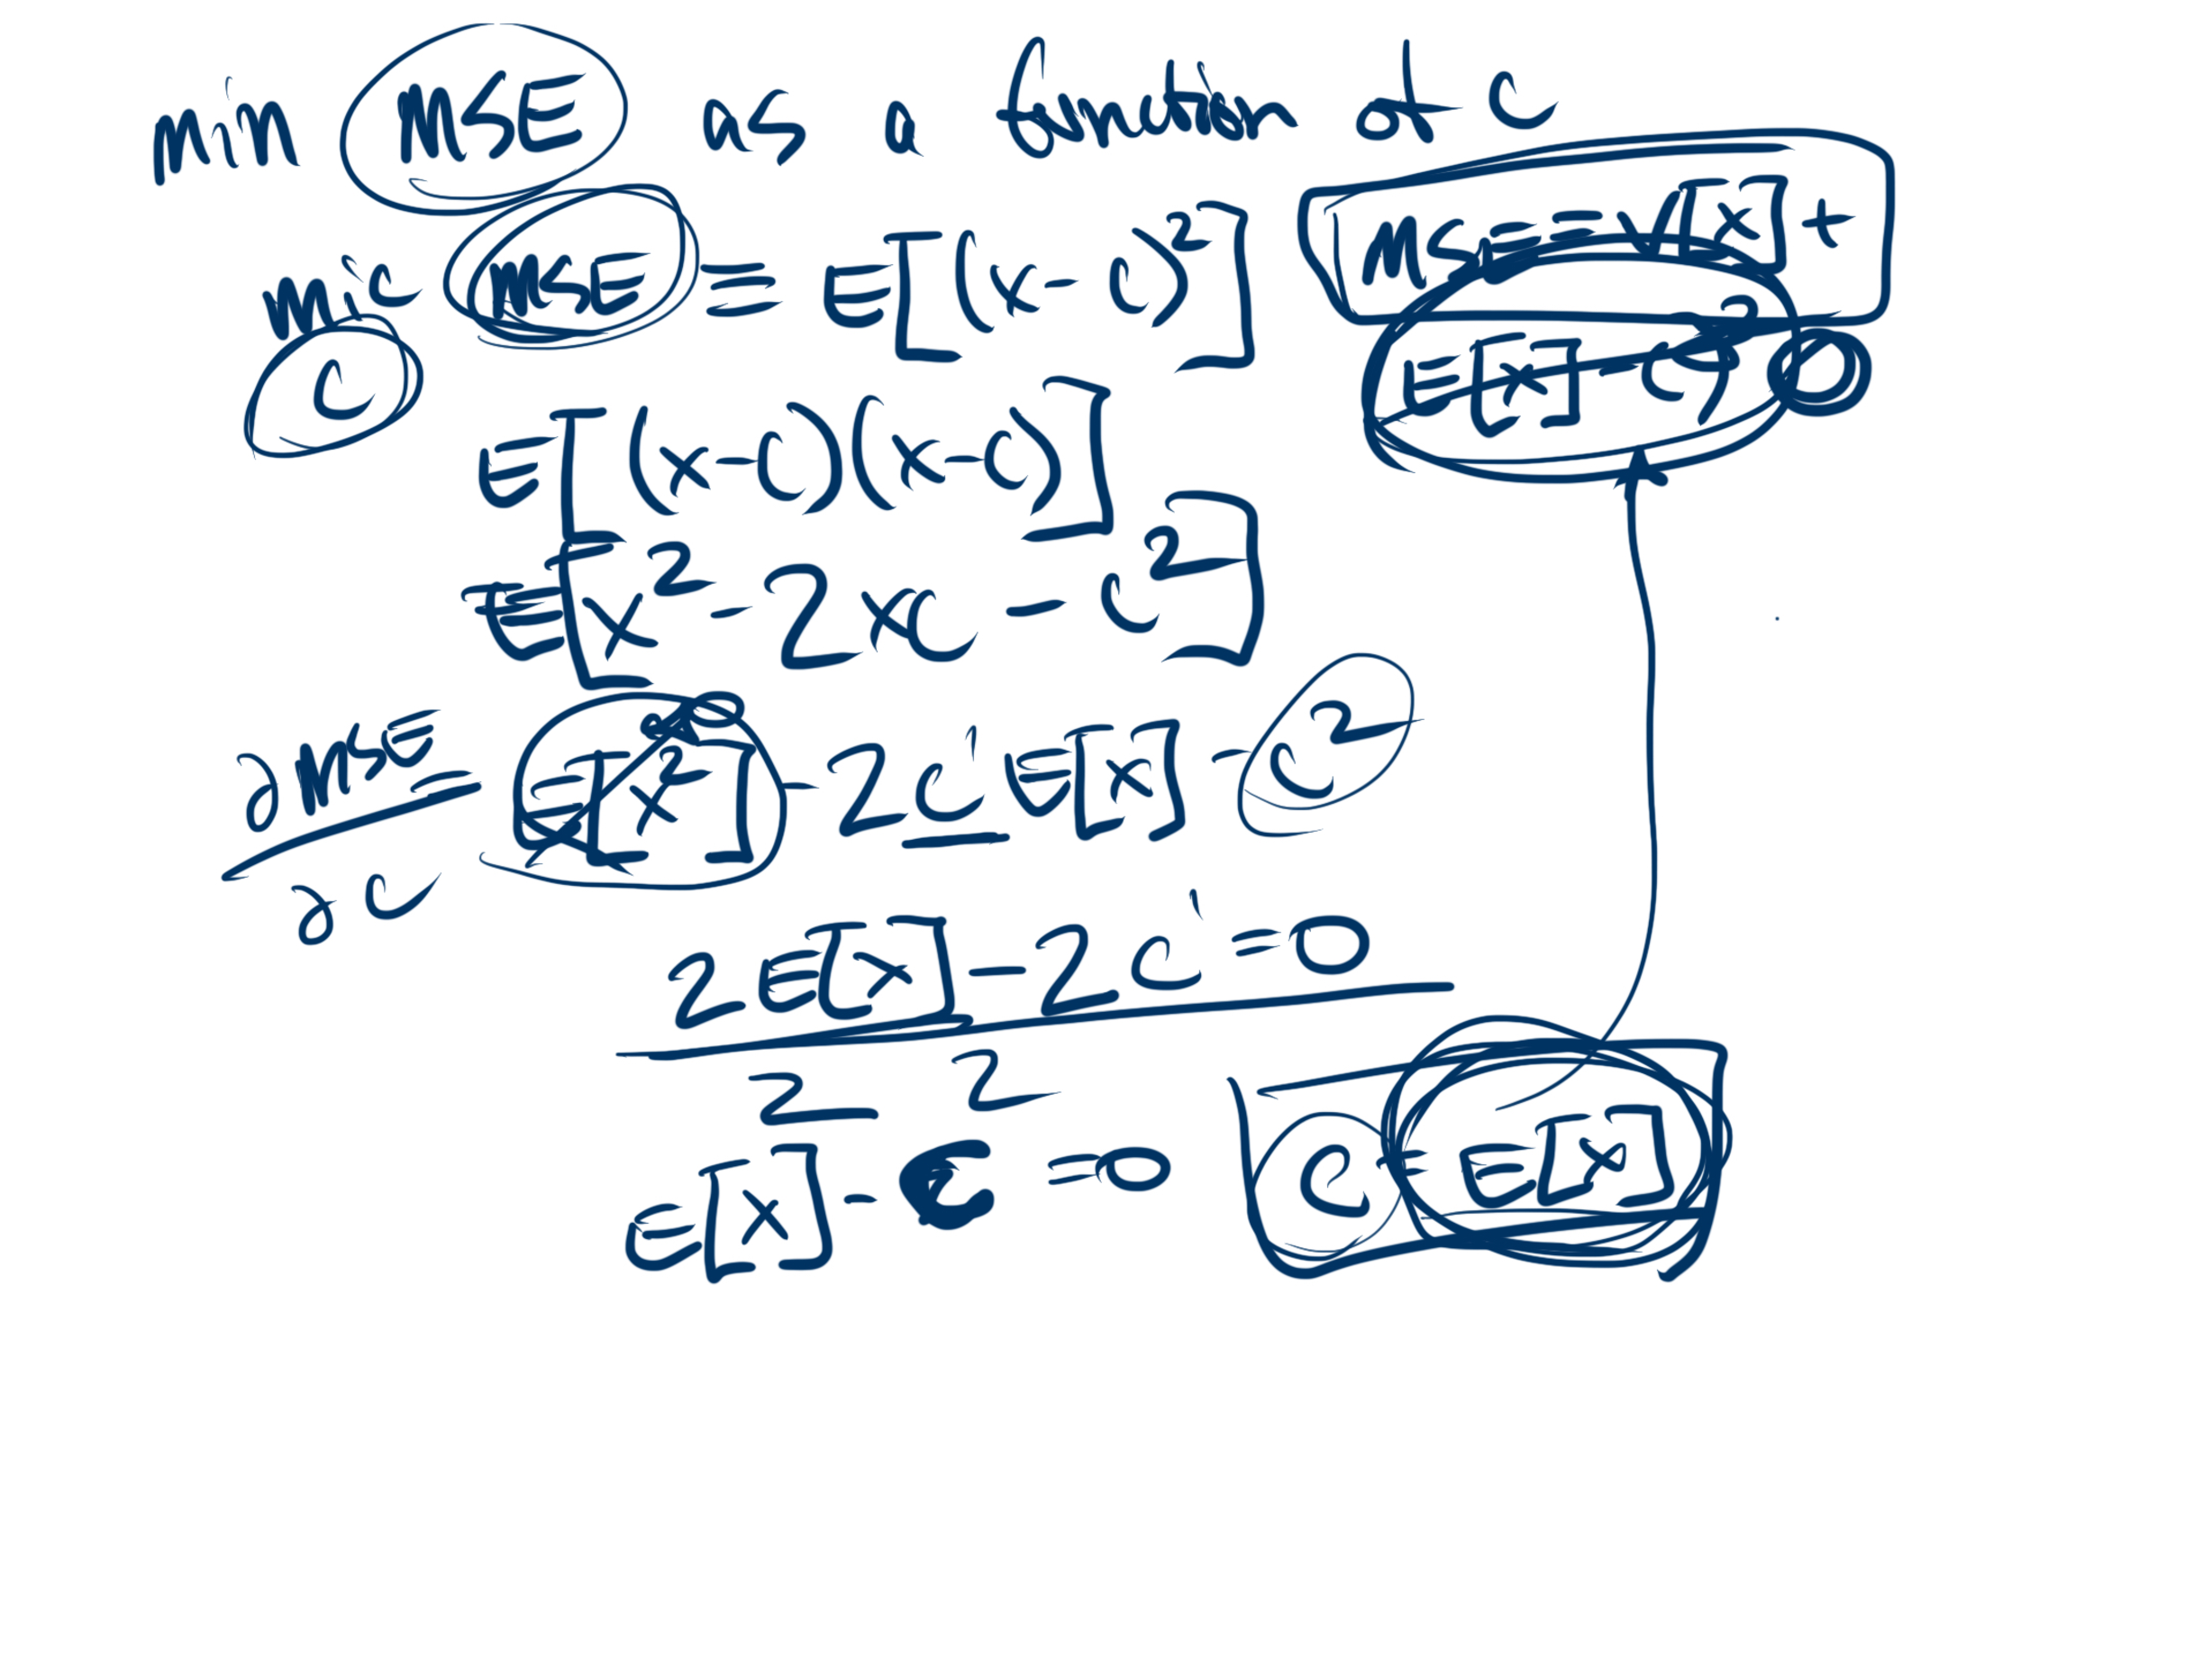
\includegraphics[width=0.3\linewidth]{images/Mean_Squared_Error_2}}
\end{frame}


 
 \section{Covariance and Correlation}
 \section{Measuring Linear Dependency}

 \begin{frame}
   \frametitle{Understanding Relationships}

   Most of the really important questions in data science are about
   \textit{relationships}.
   
   \begin{itemize}
   \item Bitterness of coffee \pause
   \item Roasting temperature and time 
   \end{itemize}

   \note[item]{If I knew everything about the marginal distribution of
     bitterness by itself, maybe I could publish a blog post.} 
   \note[item]{But, if I can understand how several variables relate
     to one another, I can do more useful things than write a
     blog-post -- I can change my world and drink better coffee.
     I could (a) Generate hypotheses; (b) Make predictions of
     bitterness for different roast profiles; (c) Maybe build a new
     coffee theory; or (d) Drink better coffee.
 }
\end{frame} 

\begin{frame}[standout]
  How can we make sense of the wide variety of relationships among
  variables?
\end{frame}


\begin{frame}
  \frametitle{The Joint Distribution}
  \centering
  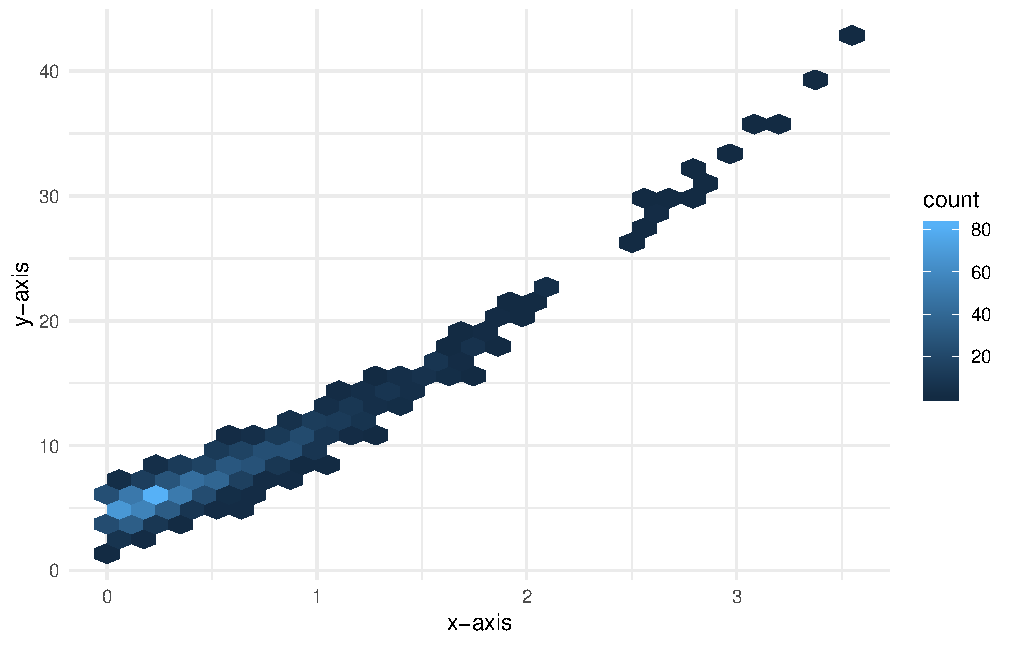
\includegraphics[width = \linewidth]{images/hex.pdf}
  
  
  \note[item]{One answer is the joint distribution. This fully
    describes the relationship between random variables} 
  \note[item]{But: (1) It's a lot of information; (2) It is
    information that doesn't come as a part of our starter-pack -- we
    are not provided a manual that has the joint distribution in it;
    (3) Somestimes, even \textit{with} data, these joint distributions
    can be difficult to estiamte.} 
  \note[item]{We really need tools that are easier to work with} 
\end{frame}

\begin{frame}
  \frametitle{Measuring Dependency}
  
  A good first question about two random variables: 
  
  \begin{center}{ \textit{How strong is the relationship?} }\end{center}
  
  Two common tools to answer this question:
  \begin{itemize}
  \item Covariance
  \item Correlation
  \end{itemize}
\end{frame}

\begin{frame}
  \frametitle{Intuition for Covariance}
  
  $$\cov(X,Y) = \E\big[ (X - E[X]) (Y -E[Y]) \big]$$
         \center{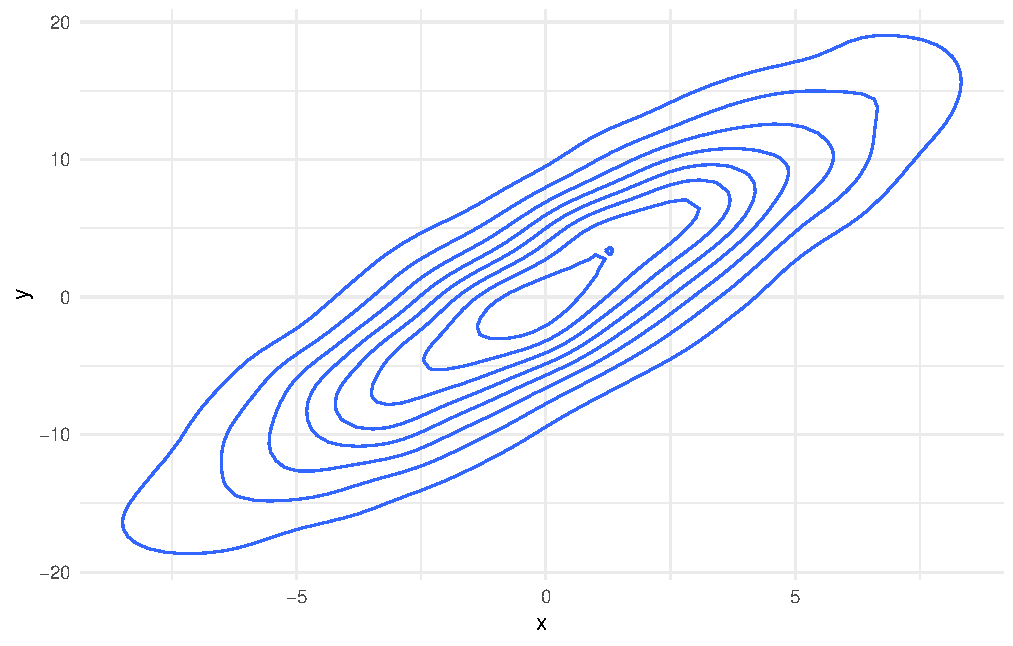
\includegraphics[width = .8\linewidth]{images/contour.pdf}}
         
\note[item]{Let's take a quick look at the covariance formula.  Just like in variance, we're looking at deviations away from a mean.  But here, we're multiplying X's deviations, by Y's deviations.}
\note[item]{Let me mark a point here, that's a high probability point.  Notice that X's deviations and Y's are positive, so when we multiply them, we get something positive.}
\note[item]{What about on the other side?  these are also high probability points.  notice that both deviations are negative, so the product is again positive.}
\note[item]{This is what we mean by two random variables varying together.  they will have positive covariance}
\end{frame}


%  \begin{frame}
%    \frametitle{Variance is Information -- Donuts}

% \paul{moving this material down to law of total variance}

%    \begin{block}{\color{gray}Variance is Information}\color{gray}
%      Variance can be parseled into two parts.
%      \begin{enumerate}\color{gray}
%      \item \textbf{Systematic Variation} is variance that we can use
%        to estimate. This variance is \textit{information} that is
%        useful.
%        \item \textbf{Stochastic Variation} is variance that is
%          random. This is variane in a process that is unattributiable,
%          or that is generated by a random process. 
%      \end{enumerate}
%    \end{block}
%  \end{frame}

\section{Reading Assignment} 
 
\begin{frame}
  \frametitle{Reading Assignment}
  \textbf{Note: This is a reading call, we're just placing it here for
    organization.}  Read \textit{Foundations of Agnostic Statistics}, pages
  59–62, stopping at Correlation.
\end{frame}


\section{Variance of Sums}
\begin{frame}
  \frametitle{Variance of Sums}
  \paul{Insert content from old section of course: 4.10 Variance of Sums}
\end{frame}

\section{Alternative Formula for Covariance}

\begin{frame}[t]
  \frametitle{Alternative Formula for Covariance}
$\cov[X,Y] = \E \big[ (X-\E[X])(Y-\E[Y]) \big]$
\end{frame}

 \section{Learnosity}

 \begin{frame}
   \frametitle{Learnosity: $\V[X - Y]$}
   You have just read theorem 2.2.3, which says, in part:
   \begin{block}{Variance of sums}
     $$\V[X + Y] = \V[X] + 2 \cov[X,Y] + \V[Y]$$
   \end{block}

   \begin{enumerate}
   \item If $X$ and $Y$ are independent — that is, $\cov[X,Y] = 0$ —
     which is larger? (a) $\V[X-Y]$; (b) $\V[X+Y]$; (c) They are the
     same. (d) We don't have enough information.
   \item If $X$ and $Y$ are not independent — that is,
     $\cov[X,Y] \neq 0$ — which is larger? (a) $\V[X-Y]$; (b) $\V[X+Y]$;
     (c) They are the same. (d) We don't have enough information.
   \end{enumerate}
 \end{frame}

 \begin{frame}
   \frametitle{Learnosity: $\V[X - Y]$ (cont.)}

   \begin{enumerate}
     \item Under what circumstances would it be possible for $V[X]$
       and $V[Y]$ to ``cancel out''?
   \item Notice that $V[X + (-1 * X)] = V[X - X] = V[0] = 0.$ Use this
     to find a simple formula for $cov[X,X]$.
   \end{enumerate} 
 \end{frame}
 
\section{Properties of Covariance Lightboard}

\begin{frame}[t]
  \frametitle{Properties of Covariance}
  For random variables $X,Y,Z,W$ and $a,b \in \R$,
\end{frame}
 
 
\begin{frame}[t]
  \frametitle{Lightboard: Linearity of Covariance}
  \textbf{Note: This is Lightboard. We're just placing it here for
    organization.}  For random variables $X, Y, Z, W$ and constants
  $a$, $b$,
   
  $cov[aX, bY] = E[aXbY] - E[aXE[BY] = abE[XY] - ab E[X]E[Y] = ab
  cov[X,Y]$
   
  $cov[X + Y, Z] = E[ (X + Y) \cdot Z ] - E[X+Y]E[Z] $
  $ = E[XZ + YZ] - (E[X] + E[Y])E[Z] = E[XZ] + E[YZ] - E[X]E[Z] -
  E[Y]E[Z]$ $ = cov[X,Z] + cov[Y,Z]$
   
  b.s.a $cov[X, Y + Z] = cov[X,Y] + cov[X,Z]$
   
  $cov[X + Y, Z + W] = cov[X, Z + W] + cov[Y, Z + W]$
  $ = cov[X,Z] + cov[X,W] + cov[Y, Z] + cov[Y,W]$
   
  \note[item]{\paul{Question for Preston: Since we
      have this nice list of properties in the theorem, provide a
      simple math problem, then just ask students multiple choice
      which of the properties they need to solve it? }}
\end{frame}
 
\section{Correlation}

\begin{frame}
  \frametitle{Correlation is Rescaled Covariance}
  
  \note[item]{Schooling is correlated with earnings.}  \note[item]{In
    general it is a stand-in for ``Is associated'' with.}
  \note[item]{But this isn't precisely correct.}

  \begin{block}{Definition 2.2.5}
    Correlation is a rescaled derivative of covariance that captures
    the \textit{linear dependence} between two random variables.
    $$
    \rho[X,Y] = \frac{\cov[X,Y]}{\sigma[X]\sigma[Y]}
    $$
  \end{block}

  Society has a plain-language usage of \textit{correlation} that is
  probably closer in usage to \textit{covariance} than to
  \textit{correlation}.
\end{frame}
 
 \begin{frame}
   \frametitle{Correlation Measures Linear Dependency}
  
   Correlation for example distributions:
   \center{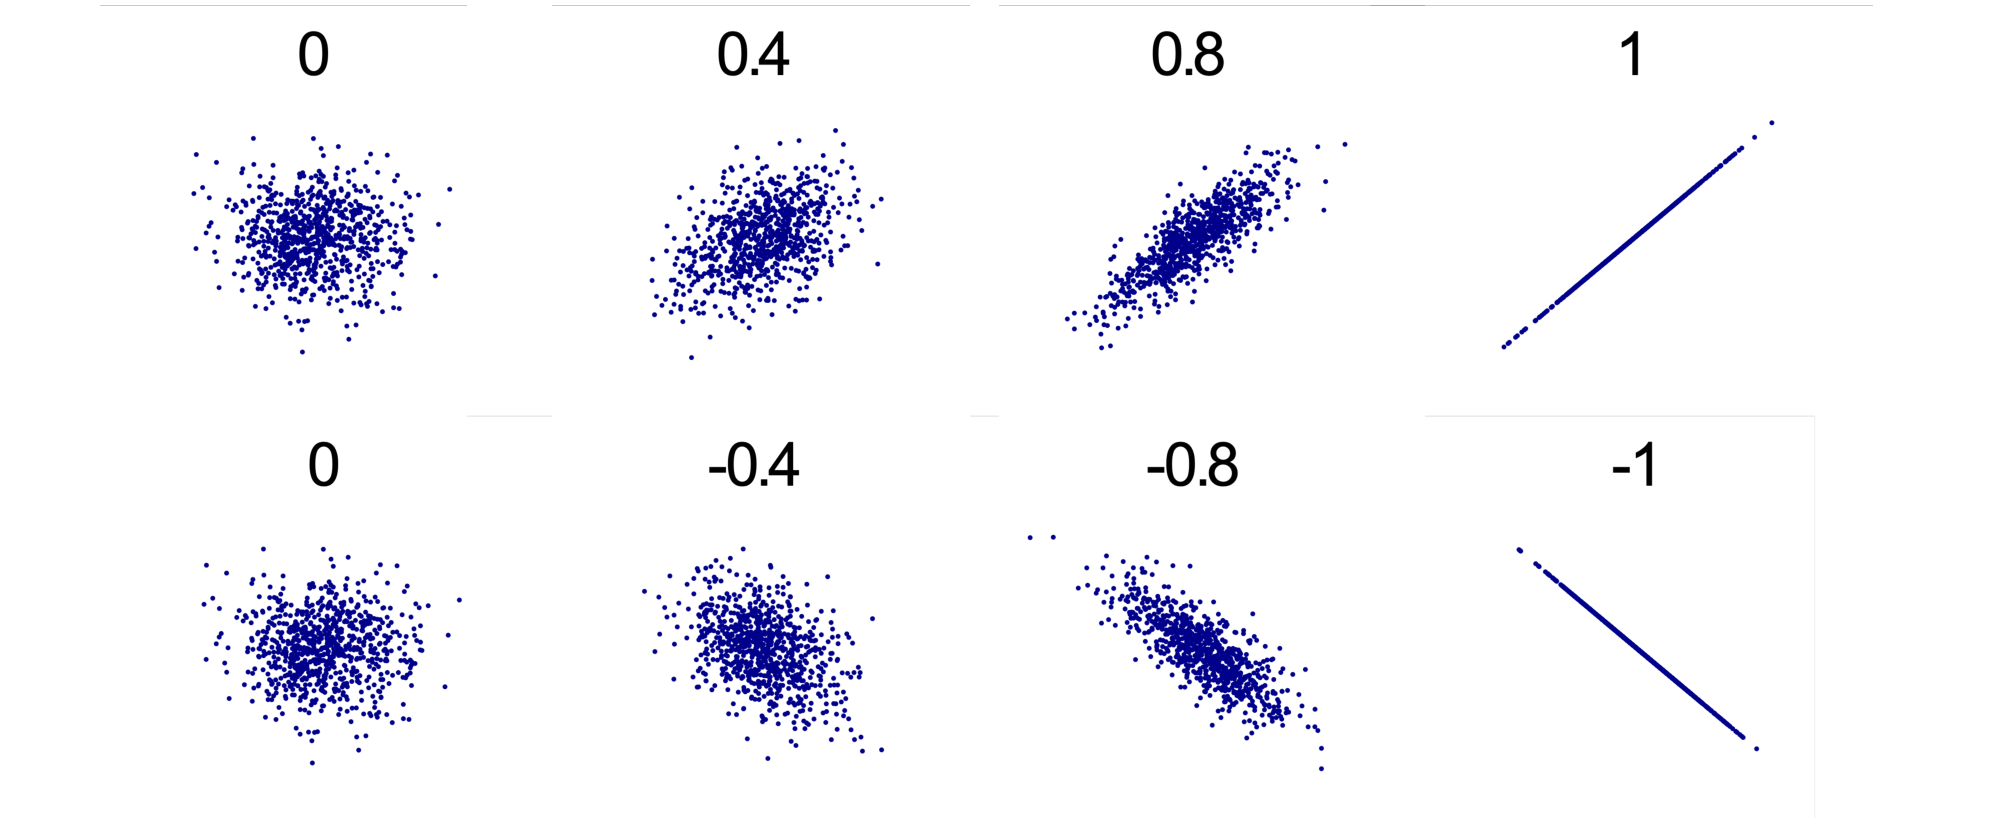
\includegraphics[width = \textwidth]{images/cor_viz}}
   Source: en.wikipedia.org/wiki/Correlation\_and\_dependence
       
   \note[item]{The presence of a correlation implies that there is
     some linear dependence between two random variables.}
   \note[item]{\paul{Here you can see some representations of
       distributions to give you an idea of what linear dependence
       looks like.}}  \note[item]{\paul{As you get close to a
       correlation of 1 or -1, the distribution becomes closer and
       closer to a line.}}
     
 \end{frame}

\begin{frame}
  \frametitle{Not All Dependency is Linear}
  
  Example distributions with zero correlation:
       \center{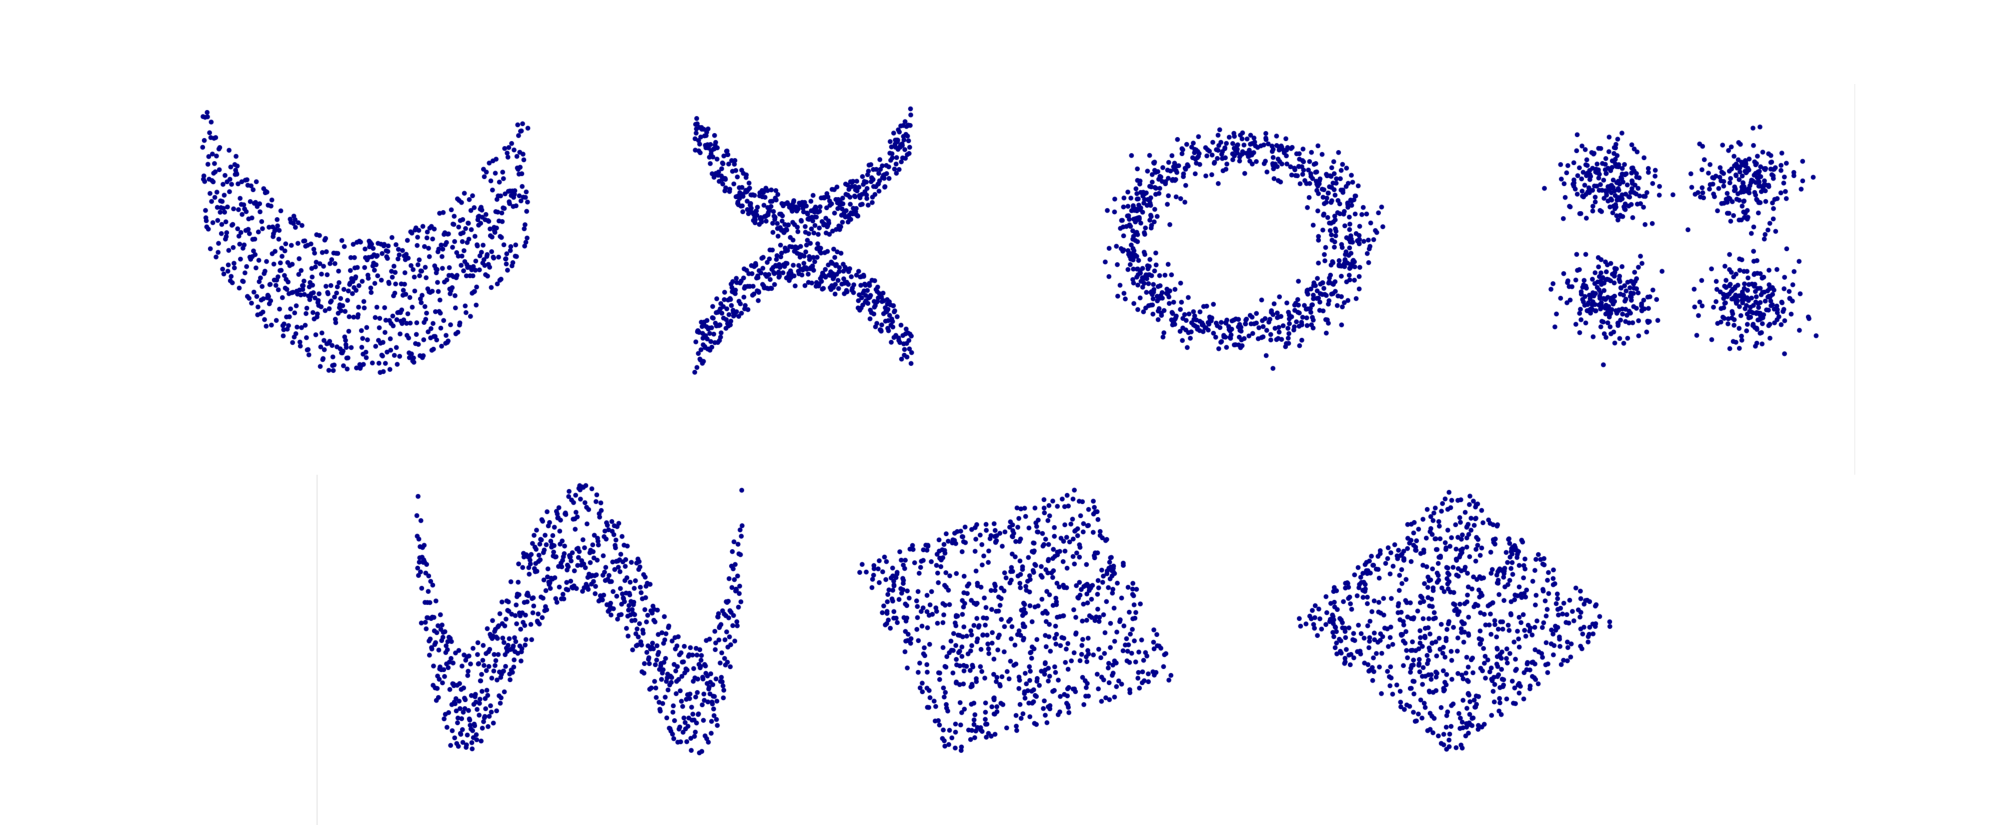
\includegraphics[width = \textwidth]{images/zero_cor}}  
       Source: en.wikipedia.org/wiki/Correlation\_and\_dependence
       \note[item]{But, the lack of a correlation (and the lack of a linear
     dependence) does not mean that there is no dependence -- does not
     mean that the random variables are independent.}
     \note[item]{\paul{Here you can see some examples where there is
         clearly a relationship - just not a linear one.}} 
\end{frame}

\section{Reading: Correlation}

\begin{frame}
  \frametitle{Reading Assignment}
  Read pages 62-65, stopping before you get to example
  2.2.9. \note[item]{Feel free to skip footnote 12. The authors are
    showing off.}
  \begin{block}{Theorem 2.2.7}
    The third and fourth bullet points can be more clearly stated.
    \begin{itemize}
    \item If $a$ and $b$ are either both positive or both negative,
      \[\rho[aX + c, bY + d] = \rho[X,Y]\]
    \item If $a$ and $b$ have opposite signs,
      \[\rho[aX + c, bY + d] = -\rho[X,Y]\]
    \end{itemize}
  \end{block}
\end{frame}

\section{Covariance, Correlation, and Independence} 

\begin{frame}
  \frametitle{Independent Variables Have Zero Correlation}
  \begin{block}{Independence $\implies \rho = 0$ }
    If $X$ and $Y$ are independent random variables, then: 
    \begin{itemize} 
    \item $\E[XY] = \E[X]\E[Y]$
    \item $\cov[X,Y] = 0$
    \item $\rho[X,Y] = 0$
    \item $\V[X + Y] = \V[X-Y] = \V[X] + \V[Y]$ 
    \end{itemize} 
  \end{block}
  \note[item]{The really neat curiosity, that we showed earlier is
    that covariance or correlation equals zero does not imply that
    the variables are independent.} 
  \note[item]{As our understanding of relationships permits
    non-linear dependencies, we're going to need a more flexible
    model. Welcome in machine learning!} 
\end{frame}

\begin{frame}
  \frametitle{Independent Variables Have Zero Correlation}
  
\end{frame} 

\section{Wrap-Up of Correlation}

\begin{frame}
  \frametitle{Wrap-Up of Correlation} 
  \textbf{Note: This is a solo-lecture. We are just placing this here
    for organization.} 

\end{frame} 

\begin{frame}
  \frametitle{Coding Activity}
  \textbf{Note: This will be a README. We're just placing it here for
    organization.}    
\end{frame}

\end{document}
